\section{Графики зависимостей}
\label{sec:graphs}

Во всех сериях, кроме специально оговорённых, используются не перекрывающиеся блоки $8 \times 8$, $p=16$, $\beta=1$ и $T_{\max}=80$. Порог $\varepsilon$ для каждого изображения фиксирован по траектории опорного запуска (значение ошибки на 10-й эпохе), поэтому внутри серии сравниваются запуски с одинаковым требованием к точности.

\subsection{Семейство A: зависимость $T$ от $\beta$}

Зависимость числа эпох от масштаба адаптивного шага приведена на рисунке~\ref{fig:family-a} и в таблице~\ref{tab:family-a}. При малых $\beta$ шаг слишком мал, и для достижения порога требуется много эпох или лимит исчерпывается. При увеличении $\beta$ обучение ускоряется, однако после некоторого значения поправки становятся неустойчивыми: ошибка растёт, и порог может не достигаться. Для разных изображений критическое значение $\beta$ различается, поскольку оно связано со спектром матрицы вторых моментов данных.

\begin{figure}[H]
	\centering
	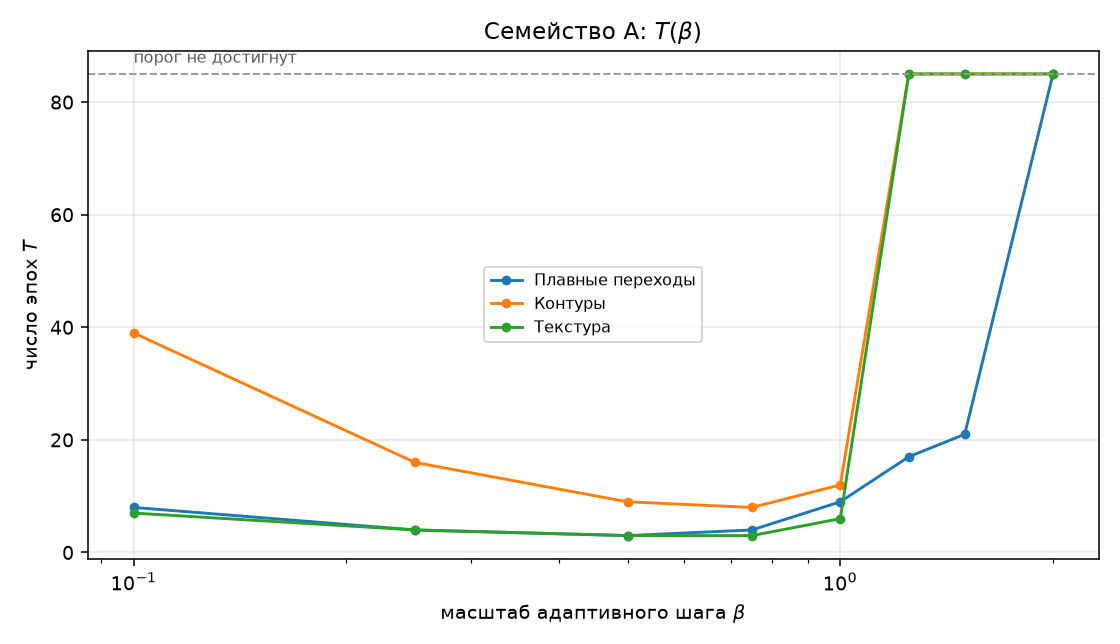
\includegraphics[width=0.82\textwidth]{family_a.png}
	\caption{Семейство A: зависимость числа эпох от масштаба адаптивного шага}
	\label{fig:family-a}
\end{figure}

\begin{table}[H]
\centering
\caption{Семейство A: число эпох при разных $\beta$}
\label{tab:family-a}
\begin{tabular}{@{}lccc@{}}
\hline
$\beta$ & Плавные переходы & Контуры & Текстура \\
\hline
0{,}1 & 8 & 39 & 7 \\
0{,}25 & 4 & 16 & 4 \\
0{,}5 & 3 & 9 & 3 \\
0{,}75 & 4 & 8 & 3 \\
1 & 9 & 12 & 6 \\
1{,}25 & 17 & --- & --- \\
1{,}5 & 21 & --- & --- \\
2 & --- & --- & --- \\
\hline
\end{tabular}
\end{table}


\subsection{Семейство B: зависимость от коэффициента сжатия}

При уменьшении $p$ коэффициент сжатия $K$ растёт, но скрытое представление сохраняет меньше независимых направлений. Зависимости числа эпох и итоговой ошибки от $K$ показаны на рисунке~\ref{fig:family-b}, числовые результаты~--- в таблице~\ref{tab:family-b}.

\begin{figure}[H]
	\centering
	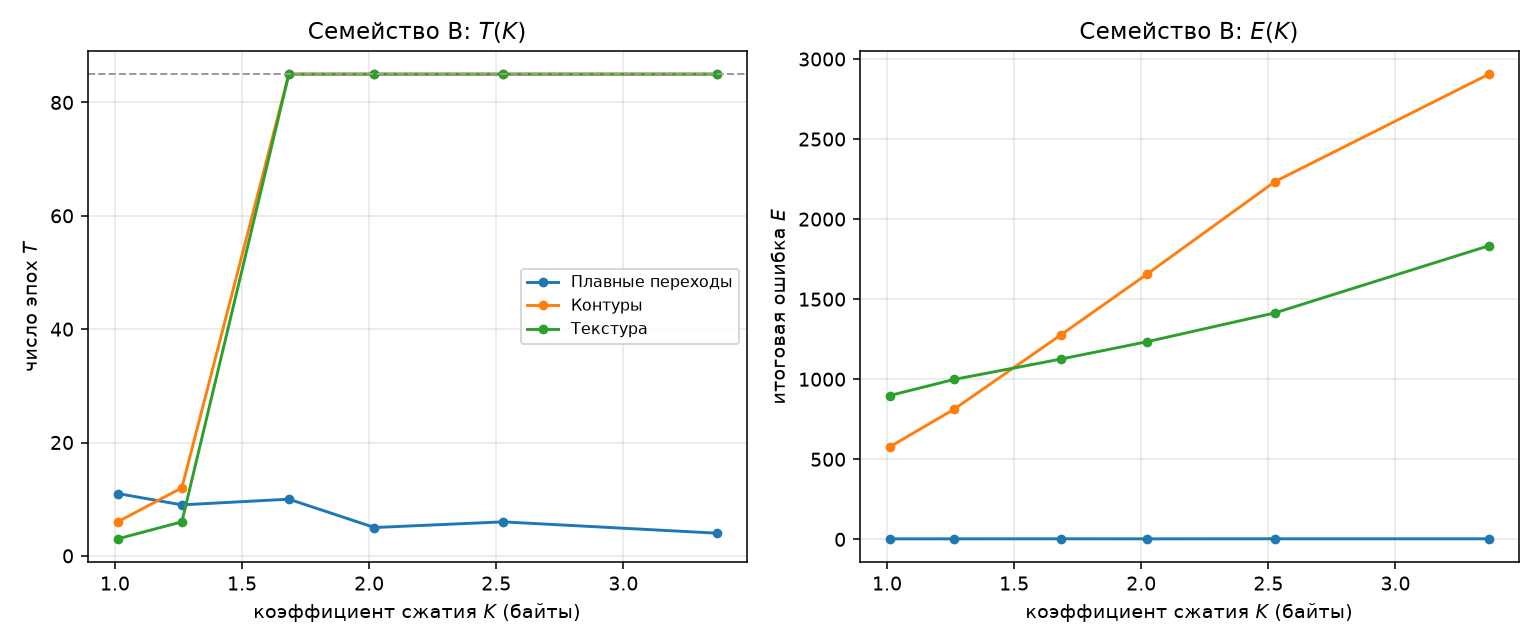
\includegraphics[width=0.98\textwidth]{family_b.png}
	\caption{Семейство B: зависимости $T(K)$ и $E(K)$}
	\label{fig:family-b}
\end{figure}

\begin{table}[H]
\centering
\caption{Семейство B: число эпох при разных $p$ и $K$}
\label{tab:family-b}
\begin{tabular}{@{}lcccc@{}}
\hline
$p$ & $K$ & Плавные переходы & Контуры & Текстура \\
\hline
6 & 3{,}368 & 4 & --- & --- \\
8 & 2{,}526 & 6 & --- & --- \\
10 & 2{,}021 & 5 & --- & --- \\
12 & 1{,}684 & 10 & --- & --- \\
16 & 1{,}263 & 9 & 12 & 6 \\
20 & 1{,}01 & 11 & 6 & 3 \\
\hline
\end{tabular}
\end{table}


При больших $K$ (малых $p$) остаточная ошибка ограничена снизу суммой отброшенных собственных чисел матрицы вторых моментов. Если этот предел превышает $\varepsilon$, порог не достигается ни за какое число эпох; в таблице такие случаи отмечены прочерком. Для контуров и текстуры порог недостижим при $p\le12$ и достигается только при $p=16$ и $p=20$; для плавных переходов он достижим во всём диапазоне $p=6\ldots20$. С ростом $p$ ошибка для контуров и текстуры монотонно уменьшается, а число эпох при $p\ge16$ снижается. Для плавных переходов $T$ с ростом $p$ слабо увеличивается (от 4 до 11 эпох), поскольку ошибка там уже мала и определяется в основном случайным порядком обновлений, а не числом компонент. Коэффициент сжатия при этом падает. Таким образом, выбор $p$ является компромиссом между качеством и объёмом представления.

\subsection{Семейство C: зависимость от типа изображения}

Сравнение трёх изображений при индивидуальных порогах и при общей допустимой MSE приведено на рисунке~\ref{fig:family-c} и в таблице~\ref{tab:family-c}. Индивидуальные пороги выбраны из условия сопоставимости с опорными запусками; общий контроль использует одинаковую среднюю ошибку \CommonMSE{} для всех изображений.

\begin{figure}[H]
	\centering
	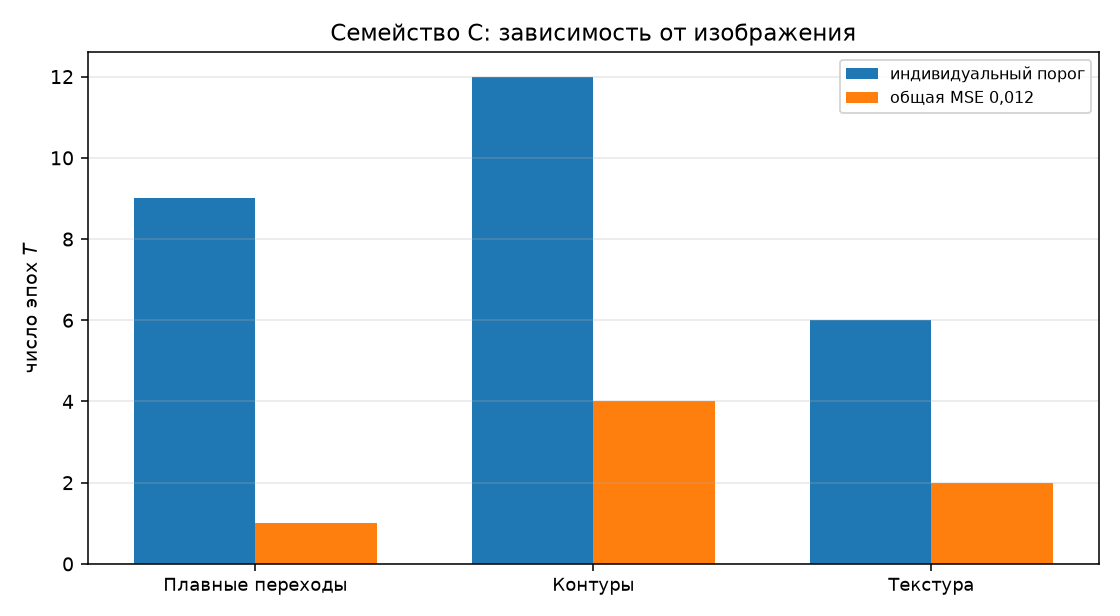
\includegraphics[width=0.78\textwidth]{family_c.png}
	\caption{Семейство C: число эпох для разных типов изображений}
	\label{fig:family-c}
\end{figure}

\begin{table}[H]
\centering
\caption{Семейство C: зависимость от типа изображения}
\label{tab:family-c}
\begin{tabular}{@{}lcccccc@{}}
\hline
Изображение & $\varepsilon_i$ & $T_i$ & $\varepsilon_{\text{общ}}$ & $T_{\text{общ}}$ & $\mathrm{MSE}_n$ & $K$ \\
\hline
Плавные переходы & 7{,}54 & 9 & 1179{,}65 & 1 & 0{,}000027 & 1{,}263 \\
Контуры & 871{,}71 & 12 & 1179{,}65 & 4 & 0{,}010536 & 1{,}263 \\
Текстура & 996{,}12 & 6 & 1179{,}65 & 2 & 0{,}009688 & 1{,}263 \\
\hline
\end{tabular}
\end{table}


Изображения с плавными переходами имеют быстро убывающий спектр: большая часть энергии сосредоточена в нескольких первых направлениях, поэтому при фиксированном $p$ отброшенная энергия мала. Контуры и текстура обладают более «тяжёлым» спектром, и для той же ошибки им требуется больше эпох. Это хорошо видно по общему порогу: при $\mathrm{MSE}_n=\CommonMSE$ плавные переходы достигают его за 1 эпоху, текстура~--- за 2, контуры~--- за 4.

Индивидуальные пороги выбраны по значению ошибки на 10-й эпохе, поэтому они сопоставимы по построению, но траектория ошибки текстуры немонотонна: после 6-й эпохи ошибка снова возрастает, из-за чего первое пересечение индивидуального порога происходит раньше ($T=6$), чем у плавных переходов ($T=9$). Поэтому для сравнения сложности изображений следует опираться на общий порог, а не на раннее пересечение индивидуального.

\subsection{Семейство D: зависимость $T$ от порога $\varepsilon$}

Число эпох до первого пересечения порога приведено на рисунке~\ref{fig:family-d} и в таблице~\ref{tab:family-d}. Все пороги проверяются по одной и той же траектории ошибки, поэтому различие в $T$ связано только с условием остановки, а не с новой инициализацией или другим порядком блоков.

\begin{figure}[H]
	\centering
	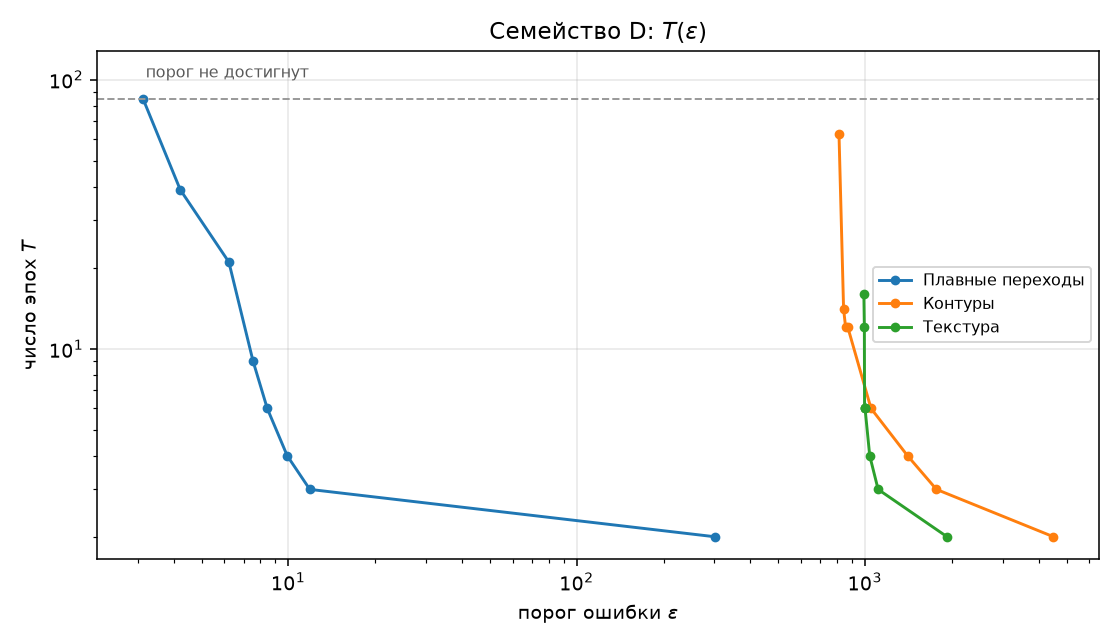
\includegraphics[width=0.82\textwidth]{family_d.png}
	\caption{Семейство D: зависимость числа эпох от порога ошибки}
	\label{fig:family-d}
\end{figure}

\begin{longtable}{@{}lll@{}}
\caption{Семейство D: число эпох при разных порогах $\varepsilon$}\label{tab:family-d}\\
\hline
Изображение & $\varepsilon$ & $T$ \\
\hline
\endfirsthead
\hline
Изображение & $\varepsilon$ & $T$ \\
\hline
\endhead
Плавные переходы & 301{,}716 & 2 \\
Плавные переходы & 11{,}865 & 3 \\
Плавные переходы & 9{,}909 & 4 \\
Плавные переходы & 8{,}447 & 6 \\
Плавные переходы & 7{,}54 & 9 \\
Плавные переходы & 6{,}216 & 21 \\
Плавные переходы & 4{,}216 & 39 \\
Плавные переходы & 3{,}131 & --- \\
\hline
Контуры & 4503{,}425 & 2 \\
Контуры & 1768{,}636 & 3 \\
Контуры & 1404{,}607 & 4 \\
Контуры & 1048{,}78 & 6 \\
Контуры & 871{,}709 & 12 \\
Контуры & 856{,}573 & 12 \\
Контуры & 842{,}641 & 14 \\
Контуры & 812{,}136 & 63 \\
\hline
Текстура & 1924{,}931 & 2 \\
Текстура & 1110{,}095 & 3 \\
Текстура & 1038{,}159 & 4 \\
Текстура & 999{,}97 & 6 \\
Текстура & 998{,}645 & 6 \\
Текстура & 996{,}124 & 6 \\
Текстура & 994{,}533 & 12 \\
Текстура & 990{,}606 & 16 \\
\hline
\end{longtable}


При приближении $\varepsilon$ к предельной достижимой ошибке $E^*$ требуемое число эпох резко возрастает: порог ниже $E^*$ не достигается при строгом условии $E<\varepsilon$. Вдали от предела зависимость близка к логарифмической, что согласуется с геометрическим затуханием ошибки в линейной модели.
